% TO-DO:  Kolmogorov complexity

\documentclass[17pt]{beamer}
\usepackage[CJKspace]{xeCJK}
%\usepackage{newtxtext,newtxmath}	% use Times Roman font
%\usefonttheme{serif}
\usefonttheme{professionalfonts}
%\setbeamertemplate{theorems}[numbered]
\setbeamertemplate{caption}{\insertcaption} 	% no `Figure' prefix before caption

\mode<presentation> {

%\usetheme{default}
%\usetheme{AnnArbor}
%\usetheme{Antibes}
%\usetheme{Bergen}
%\usetheme{Berkeley}
%\usetheme{Berlin}
%\usetheme{Boadilla}
%\usetheme{CambridgeUS}
%\usetheme{Copenhagen}
%\usetheme{Darmstadt}
%\usetheme{Dresden}
%\usetheme{Frankfurt}
%\usetheme{Goettingen}
%\usetheme{Hannover}
%\usetheme{Ilmenau}
%\usetheme{JuanLesPins}
%\usetheme{Luebeck}
\usetheme{Madrid}
%\usetheme{Malmoe}
%\usetheme{Marburg}
%\usetheme{Montpellier}
%\usetheme{PaloAlto}
%\usetheme{Pittsburgh}
%\usetheme{Rochester}
%\usetheme{Singapore}
%\usetheme{Szeged}
%\usetheme{Warsaw}

%\usecolortheme{albatross}
%\usecolortheme{beaver}
%\usecolortheme{beetle}
%\usecolortheme{crane}
%\usecolortheme{dolphin}
%\usecolortheme{dove}
%\usecolortheme{fly}
%\usecolortheme{lily}
%\usecolortheme{orchid}
%\usecolortheme{rose}
%\usecolortheme{seagull}
%\usecolortheme{seahorse}
%\usecolortheme{whale}
%\usecolortheme{wolverine}

%\setbeamertemplate{footline} % To remove the footer line in all slides uncomment this line
%\setbeamertemplate{footline}[page number] % To replace the footer line in all slides with a simple slide count uncomment this line
\setbeamertemplate{navigation symbols}{} % To remove the navigation symbols from the bottom of all slides uncomment this line
}

\usepackage{graphicx} % Allows including images
\usepackage{verbatim} % comments
% \usepackage{tikz-cd}  % commutative diagrams
% \newcommand{\tikzmark}[1]{\tikz[overlay,remember picture] \node (#1) {};}
% \usepackage{booktabs} % Allows the use of \toprule, \midrule and \bottomrule in tables
% \usepackage{amssymb}  % \leftrightharpoons
\usepackage{wasysym} % frownie face

\newcommand{\vect}[1]{\boldsymbol{#1}}
\newcommand*\sigmoid{\vcenter{\hbox{
\includegraphics{sigmoid.png}}}}

\makeatletter
\renewcommand{\boxed}[1]{\fbox{\m@th$\displaystyle\scalebox{0.9}{#1}$} \,}
\makeatother

%---------------------------- make slide margin narrower --------------------------------
\newcommand\Wider[2][3em]{%
	\makebox[\linewidth][c]{%
		\begin{minipage}{\dimexpr\textwidth+#1\relax}
			\raggedright#2
		\end{minipage}%
}%
}

%----------------------------------------------------------------------------------------
%	TITLE PAGE
%----------------------------------------------------------------------------------------

\title[AGI theory]{Some basic notions in AGI \\ \& my theory} % The short title appears at the bottom of every slide, the full title is only on the title page

\author{YKY 甄景贤} % Your name
\institute[] % Your institution as it will appear on the bottom of every slide, may be shorthand to save space
{
Independent researcher, Hong Kong \\ % Your institution for the title page
\medskip
\textit{generic.intelligence@gmail.com} % Your email address
}
\date{\today} % Date, can be changed to a custom date

\begin{document}

\frame{\titlepage}

\begin{frame}
\frametitle{Talk summary}
\tableofcontents
\end{frame}

%---------------- this is for when you're using \part's ----------------------------------
%\begin{frame}
%\frametitle{Summary}
%
%{\usebeamerfont*{frametitle} Part I %\usebeamercolor[fg]{frametitle}
% ~ ~ ~ Deep reinforcement learning}
%%\tableofcontents[part=1]
%
%\vspace{1.5cm}
%{\usebeamerfont*{frametitle} Part II %\usebeamercolor[fg]{frametitle}
% ~ ~ ~ Logical structure}
%%\tableofcontents[part=2]
%\end{frame}

%----------------------------------------------------------------------------------------
%	PRESENTATION SLIDES
%----------------------------------------------------------------------------------------

%------------------------------------------------

%\part{title}

\section[Section]{What is inductive bias? ``No free lunch'' theorem}
\frame{\sectionpage}

\begin{frame}
\frametitle{The goal of machine learning}
\begin{itemize}
	\item The goal of machine learning is to search in a \textbf{space} of learning machines, those machines that satisfy certain criteria
	\item For example, among the neural networks of a certain size and shape, find the weights that satisfy an \textbf{objective function}
\end{itemize}
\end{frame}

\begin{frame}
\frametitle{AI Winter}
\begin{itemize}
	\item Generally speaking, bottleneck problem of AI = {\color{red}\textbf{search space too large}}, thus learning too slow
	\item Historically, ``AI Winter'' occurred because \textbf{logic-based} AI learning suffers from combinatorial explosion, and we lacked workable \textbf{heuristics} to tackle it
\end{itemize}
\end{frame}

\begin{frame}
\frametitle{Inductive bias}
\begin{itemize}
	\item Every learning algorithm has its \textbf{inductive bias}
	\item That is to say, some regions of the search space would \textbf{not} be searched
	\item Bias makes learning faster
	\item But if bias is too strong, the space containing the solution would be cut off \\
	``Throw the baby out with the water''
\end{itemize}
\end{frame}

\begin{frame}
\frametitle{``No free lunch'' theorem}
\fontsize{16}{15}\selectfont
\begin{itemize}
	\item When search space has no \textit{a priori} structure, any inductive bias would be {\color{red}\textbf{good at some problems while bad at others}} --- ``no free lunch''
	\item For example, vision has the structure of 3D Euclidean geometry, thus the human visual cortex may have inductive bias for this invariance
	\item Or, human cognition has ``logical'' structure, using this inductive bias may accelerate machine learning of human intelligence
\end{itemize}
\end{frame}

\begin{frame}
\frametitle{Kolmogorov complexity}
\fontsize{16}{15}\selectfont
\begin{itemize}
	\item is {\color{red}\textbf{incomputable}}, but {\color{red}\textbf{approximable}}
	\item The {\color{red}\textbf{semantic distance metric}} between logic propositions is related to it, where one logic deduction step corresponds to 1 unit of semantic distance
	\item Find a set of logic rules, that \textbf{explains} the world, and not deduce false facts, and \# of rules cannot be too large --- these requirements \textit{implicitly} approximate Kolmogorov complexity
\end{itemize}
\end{frame}

\section[Section]{What gives neural networks their power?}
\frame{\sectionpage}

\begin{frame}
\frametitle{Structure of a neural network}
\begin{itemize}
	\item 1 neuron is a \textbf{dot product} followed by a \textbf{non-linearity}:
	\begin{equation}
	\sigmoid \langle \vect{x}, \vect{w} \rangle
	\end{equation}	
	\item The non-linearity can take various forms, \textit{eg}:
	\begin{equation}
	\sigmoid (\xi) = \frac{1}{1 + e^{- \xi}}
	\end{equation}
\end{itemize}
\end{frame}

\begin{frame}
\frametitle{Structure of a neural network}
\begin{itemize}
	\item 1 \textbf{layer} of neurons is a matrix multiplication:
	\begin{equation}
	\sigmoid( \; W \cdot \vect{x} \; )
	\end{equation}	
	\item A neural \textbf{network} is the function \textbf{composition} $(f \circ f)$ of many layers:
	\begin{equation}
	[ \sigmoid W ]^L \; \vect{x}
	\end{equation}	
\end{itemize}
\end{frame}

\begin{frame}
\frametitle{Properties of neural networks}
\begin{itemize}
	\item An NN is a function with many {\color{red}\textbf{parameters}}
	\item It is a \textbf{universal function approximator} [Cybenko 1989]
	\item Its proof can be traced to Weierstrauss's approximation theorem (1885): any continuous function can be uniformly approximated by polynomials
	\item But the proof is {\color{red}independent of depth}
\end{itemize}
\end{frame}

\begin{frame}
\frametitle{Power of NNs comes from depth}
\begin{itemize}
	\item Suppose $\sigmoid W \vect{x}$ is a \textit{cubic} polynomial
	\item Adding each layer is equivalent to:
	\begin{equation}
	 (\mbox{polynomial} \circ \mbox{polynomial})
	\end{equation}
	\item Thus, the resulting polynomial has total degree = $3^L$
	\item In other words, total degree grows  {\color{red}\textbf{exponentially}}
\end{itemize}
\end{frame}

\begin{frame}
\frametitle{Power of NNs comes from depth}
\begin{itemize}
	\item \textbf{Fundamental theorem of algebra}: polynomial \textbf{degree} = zero-crossings of curve with $x=0$
	\begin{equation}
	\vcenter{\hbox{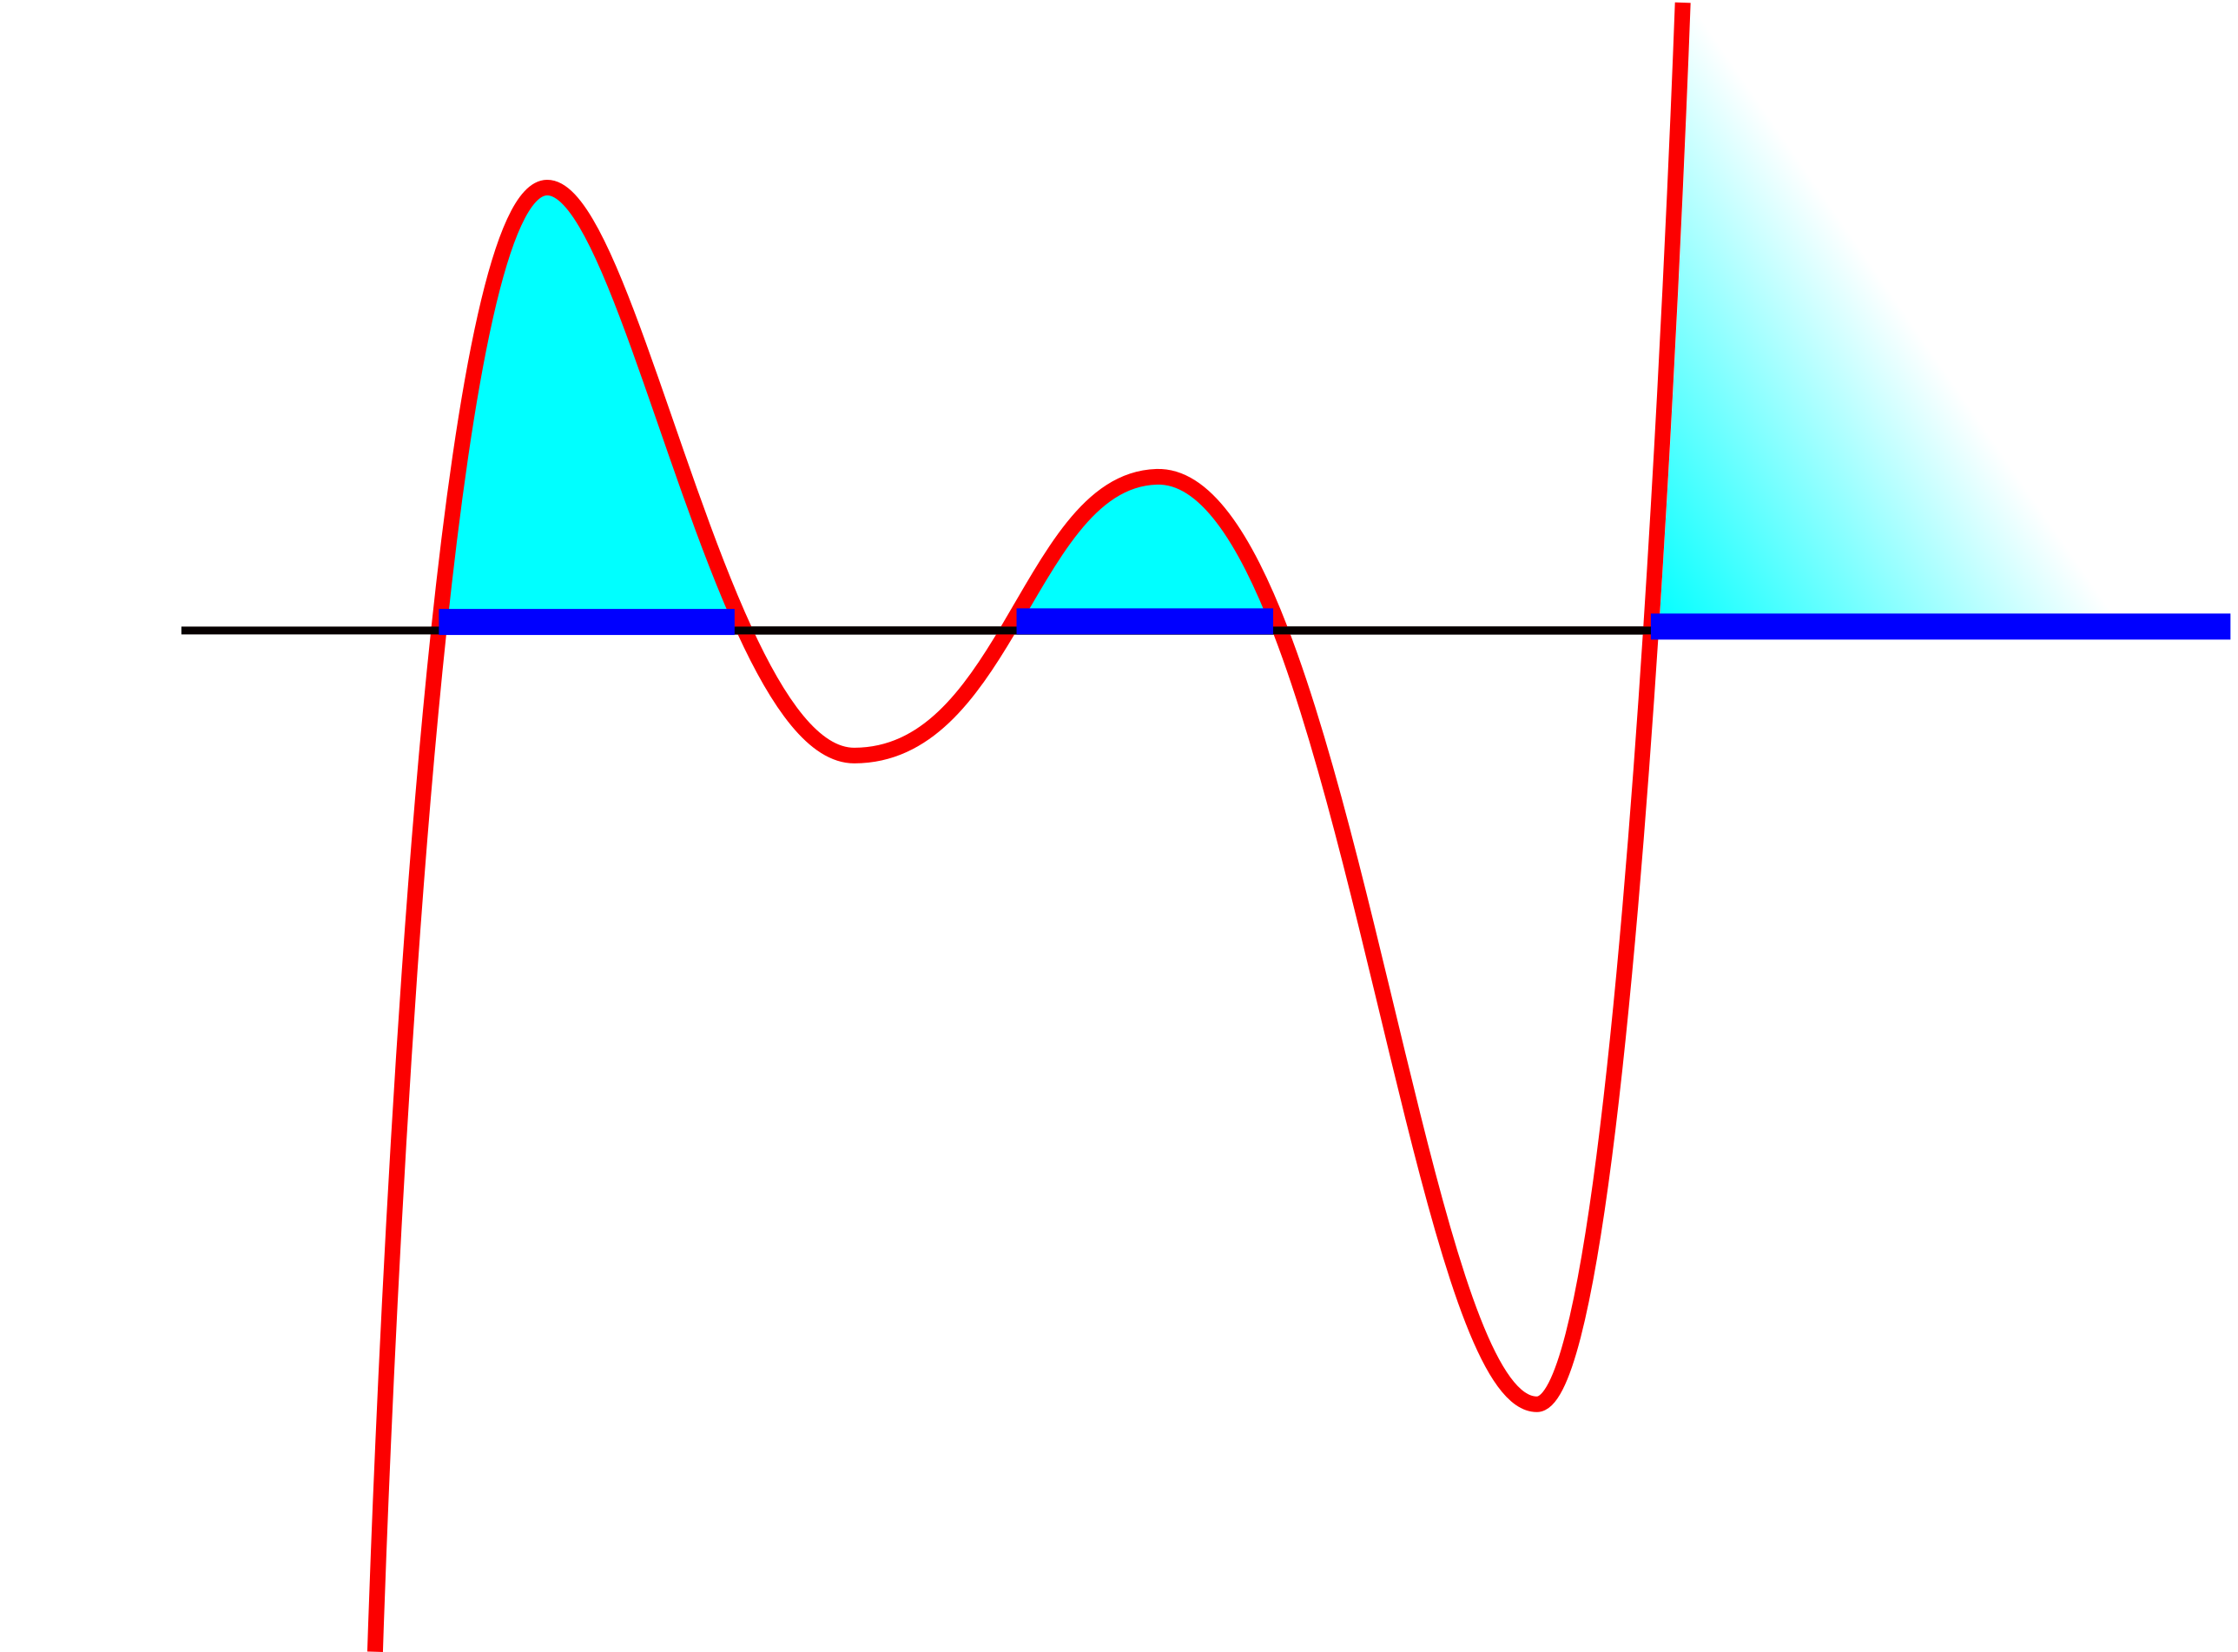
\includegraphics[scale=0.4]{zero-crossings.png}}}
	\end{equation}
	\item In higher dimensions: {\color{red}how many pieces} does a surface carve up the space
\end{itemize}
\end{frame}

\begin{frame}
\frametitle{Power of NNs comes from depth}
\begin{itemize}
	\item Same idea as \textbf{VC-dimension} [Vapnik–Chervonenkis 1971] 
	\item VC-dim = max \# pieces the ambient space is \textit{shattered} by a family of functions
	\item My conjecture: VC-dim of multi-layer NN grows exponentially as \# layers
	\item Contradicts with current bound = $O(W \log W)$ where $W$ = total \# parameters; I will investigate further
\end{itemize}
\end{frame}

\begin{frame}
\frametitle{Power of NNs comes from depth}
\begin{itemize}
	\item The {\color{red}\textbf{exponential growth}} of VC-dim means that NNs can represent highly complex \textbf{families} of functions
	\item and with a relatively small \# of parameters, which can be implemented on a computer
\end{itemize}
\end{frame}

\begin{frame}
\frametitle{Revelation from convolutional NNs}
\begin{itemize}
	\item Yann LeCun in 1989 invented \textbf{ConvNets}, which revolutionized machine vision, and got him a Turing Award
	\begin{equation}
	\nonumber
	\vcenter{\hbox{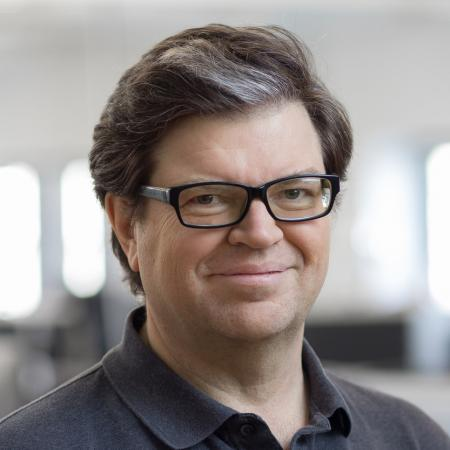
\includegraphics[scale=0.25]{Yann-LeCun.jpg}}}
	\end{equation}
\end{itemize}
\end{frame}

\begin{frame}
\frametitle{Revelation from convolutional NNs}
\fontsize{15}{15}\selectfont
\begin{itemize}
	\item CNN replaces the conventional \textbf{dot product} with the \textbf{covolutional product}:
	\begin{equation}
	\boxed{\mbox{dot product}} \quad \sigmoid \langle \vect{x}, \vect{w} \rangle \rightsquigarrow \sigmoid( f * g ) \quad \boxed{\mbox{convolution}}
	\end{equation}
	\item The convolution has {\color{red}\textbf{translation invariance}}, which is suitable for vision:
	\begin{equation}
	T_x(f) * g = T_x( f * g )
	\end{equation}
	\item This is an \textbf{inductive bias}, that makes learning faster
\end{itemize}
\end{frame}

\begin{frame}
\frametitle{Revelation from convolutional NNs}
\begin{itemize}
	\item Actually \textbf{vision} obeys \textbf{affine} invariance, \textit{ie}: translations, rotations, dilations, ...
	\item It seems that merely translational invariance yields enough \textbf{acceleration} such that CNNs surpassed human vision performance in 2012
	\item Thus we see that \textbf{inductive bias} is still useful in deep learning
\end{itemize}
\end{frame}

\section{Turing machines and universal logic}
\frame{\sectionpage}

\begin{frame}
\frametitle{Finite state machines}
\begin{itemize}
	\item Finite state machines are usually defined by tuples (skipped here), \textit{eg}:
	\begin{equation}
	\vcenter{\hbox{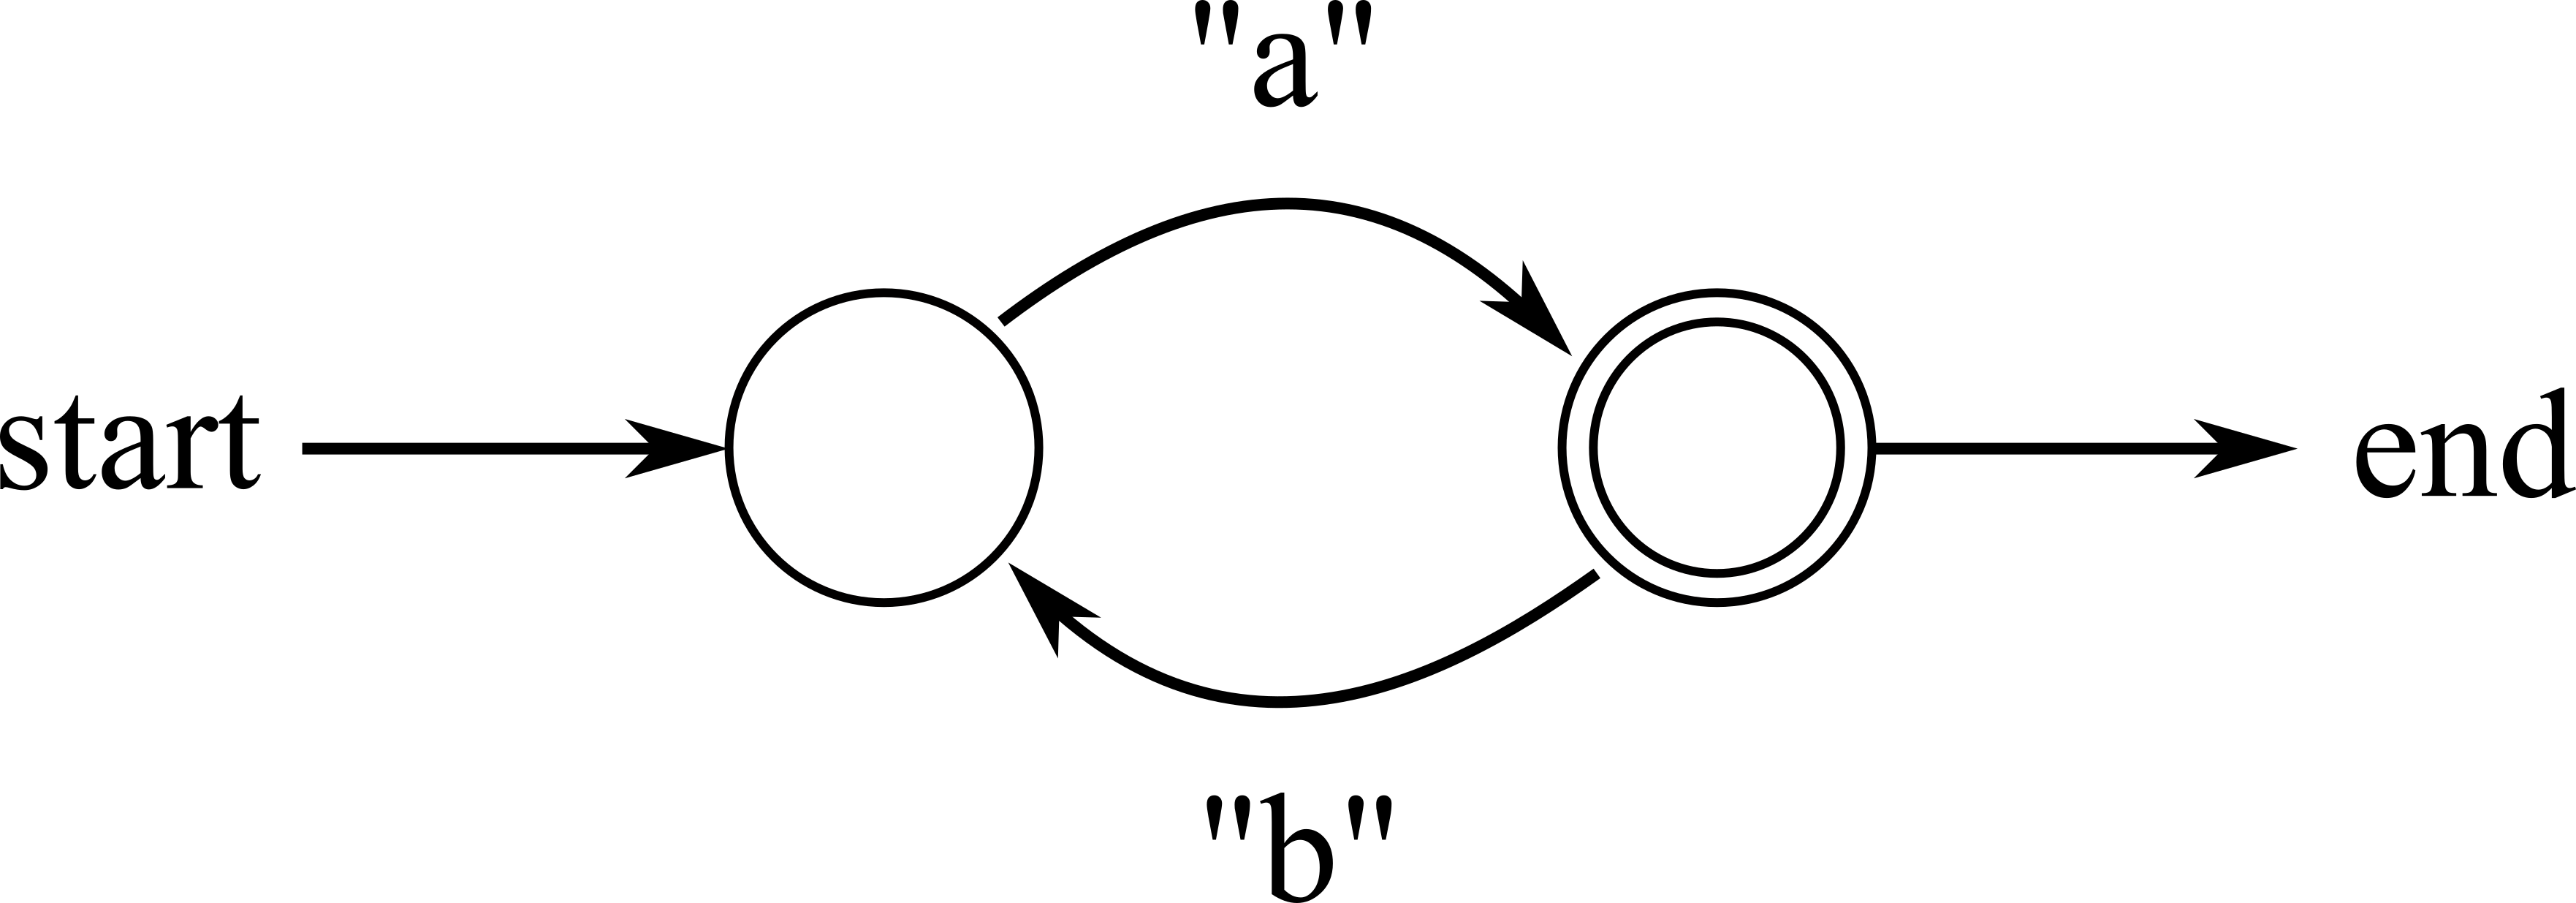
\includegraphics[scale=0.7]{finite-state-machine.png}}}
	\end{equation}
	\item This automata {\color{red}\textbf{accepts}} strings like ``a'', ``aba'', ``ababa...''
\end{itemize}
\end{frame}

\begin{frame}
\frametitle{Finite state machines}
\Wider[1em]{
\begin{itemize}
	\item FSMs can accept strings of the form $\mbox{a}^m \mbox{b}^n$, where $m$ and $n$ are different
	\item But they can't recognize $\mbox{a}^k \mbox{b}^k$ as they have no way to ``remember'' how many times $k$ is
	\item The \textbf{languages} accepted by FSMs are called \textbf{regular languages}
	\item Formulated in 1950s by Noam Chomsky (computer scientist + linguist, now a leftist critic of US politics)
\end{itemize}
}
\end{frame}

\begin{frame}
\frametitle{Turing machines}
	Turing machine = finite state machine + infinite {\color{red}\textbf{memory tape}} (each state can read/write 1 symbol)\\
	\begin{equation}
	\label{fig:Turing-machine}
	\includegraphics[scale=0.6]{../AGI-16/Turing-machine.png}
	\end{equation}
\end{frame}

\begin{frame}
\frametitle{Turing machines}
\begin{itemize}
	\item Finite state machine + infinite tape = can compute all computable functions, \textit{ie}, \textbf{Church-Turing hypothesis}
	\item Turing machines are \textbf{equivalent} to: $\lambda$-calculus, combinatory logic, cellular automata, game of life, recurrent neural networks, ... \textit{etc}
\end{itemize}
\end{frame}

\begin{frame}
\frametitle{Alan Turing (1912-1954)}
\begin{itemize}
	\item Turing was a man very much ahead of his time
	\item He considered neurons as learning machines
	\item Also considered evolutionary algorithms
	\item In 1940s there were no computers yet --- he invented them!
	\item {\color{red}He formulated the form of \textbf{all computable functions}, thus \textbf{confining} the problem of AI within a framework}
\end{itemize}
\end{frame}

\begin{frame}
\frametitle{Recurrent neural networks}
\Wider[1em]{
	Structure of RNNs can be seen as similar to (\ref{fig:Turing-machine}):
	\begin{equation}
	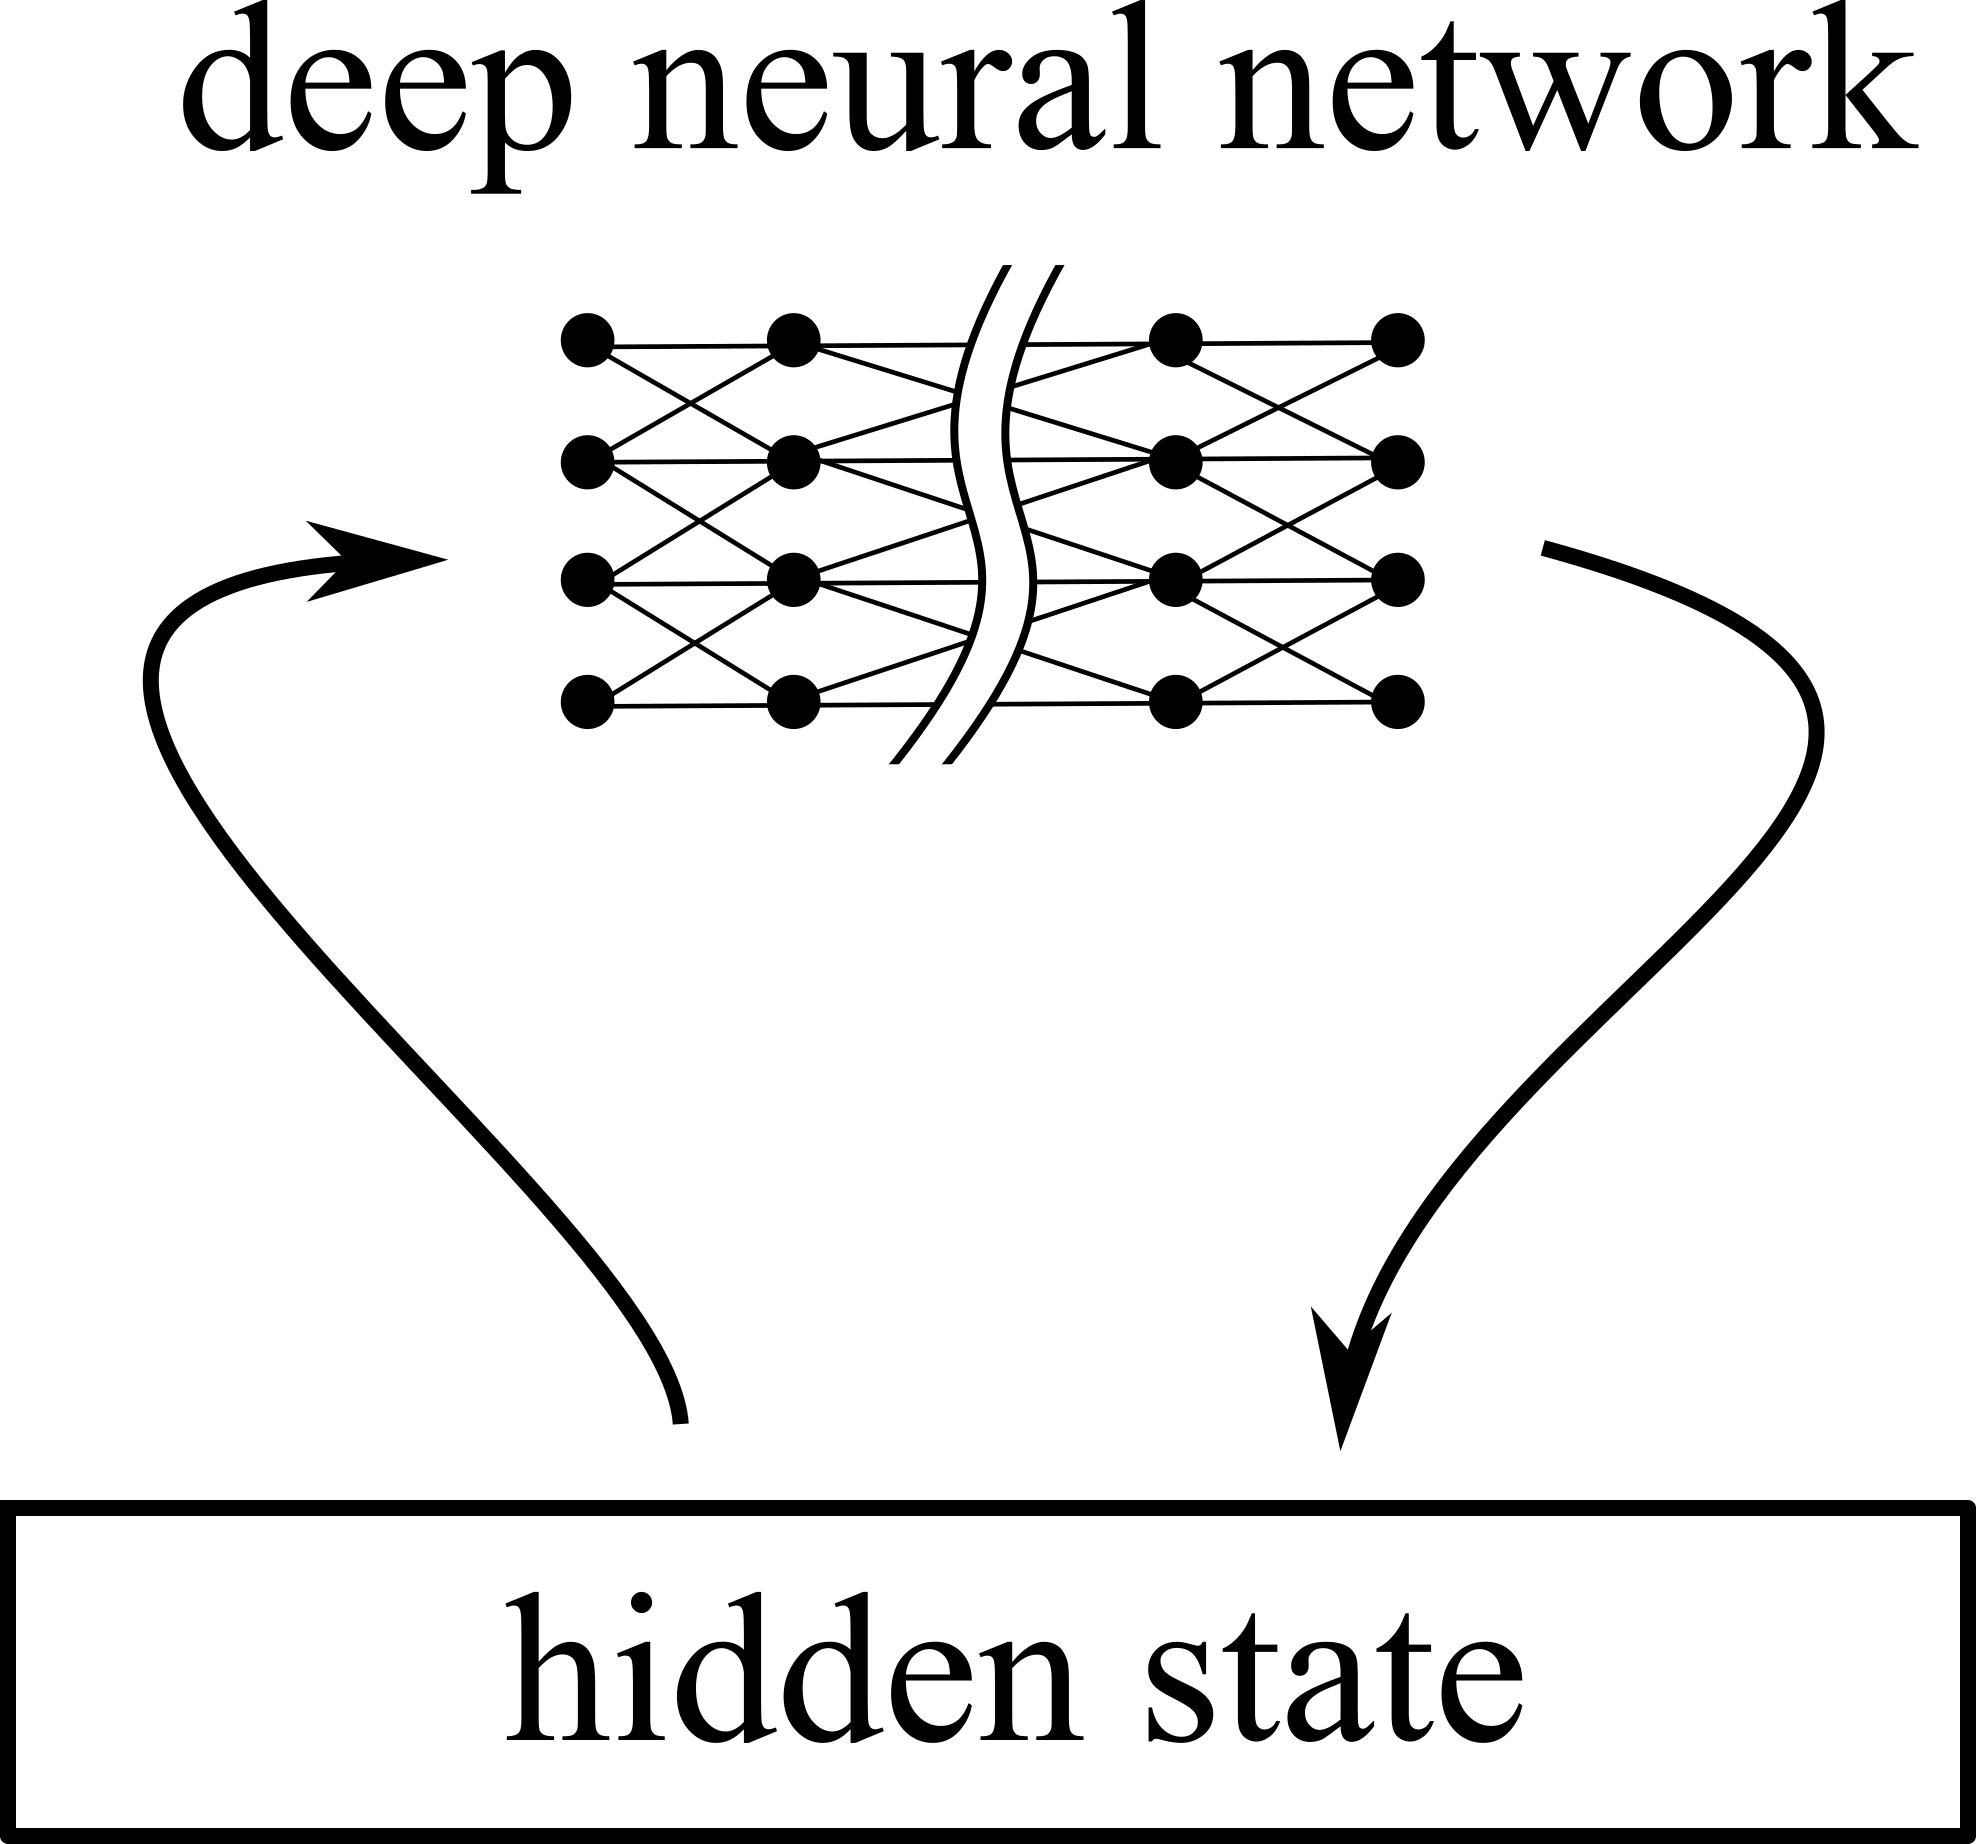
\includegraphics[scale=0.6]{RNN-as-Turing-machine.png}
	\end{equation}
	Key is that the \textbf{hidden state} can store {\color{red}\textbf{intermediate results}} of computations, enabling RNNs to be Turing-universal
}
\end{frame}

\section[Section]{Structure of classical AI systems}
\frame{\sectionpage}

\begin{frame}
\frametitle{John McCarthy (1927-2011)}
\begin{itemize}
	\item ``Father of AI''
	\item Held the first AI conference in 1956 in Dartmouth
	\item Pioneered the use of {\color{red}\textbf{mathematical logic}} as \textbf{knowledge representation} in AI
	\item In later years he studied \textbf{term rewriting systems}, a more \textbf{generalized} form of logic
\end{itemize}
\end{frame}

\begin{frame}
\frametitle{The world of logical structures}
\Wider[2em]{
\includegraphics[scale=0.43]{../2018/world-of-logical-structures.png}}
\end{frame}

\begin{frame}
\frametitle{Propositional vs predicate logic}
\Wider[1em]{
\fontsize{16}{15}\selectfont\fontsize{16}{15}\selectfont
\begin{itemize}
	\item The important distinction is between \textbf{propositional} and first-order \textbf{predicate} logic
	\item In propositional logic, {\color{red}propositions don't have \textbf{internal structure}} \\
	\hspace{3cm} $P_1 =$ ``It rained yesterday'' \\ \hspace{3cm} $P_2 =$ ``It's raining today''
	\item Predicate logic: $P_3 =$ rain(New York, today)
	\item Predicates bring about the complexity of \textbf{substitutions}
\end{itemize}
}
\end{frame}

\begin{frame}
\frametitle{Architecture of logic-based AI systems}
This cycle is as important as the \textit{Carnot cycle} in the age of steam engines:
\begin{equation}
\label{fig:LBAI-architecture}
\vcenter{\hbox{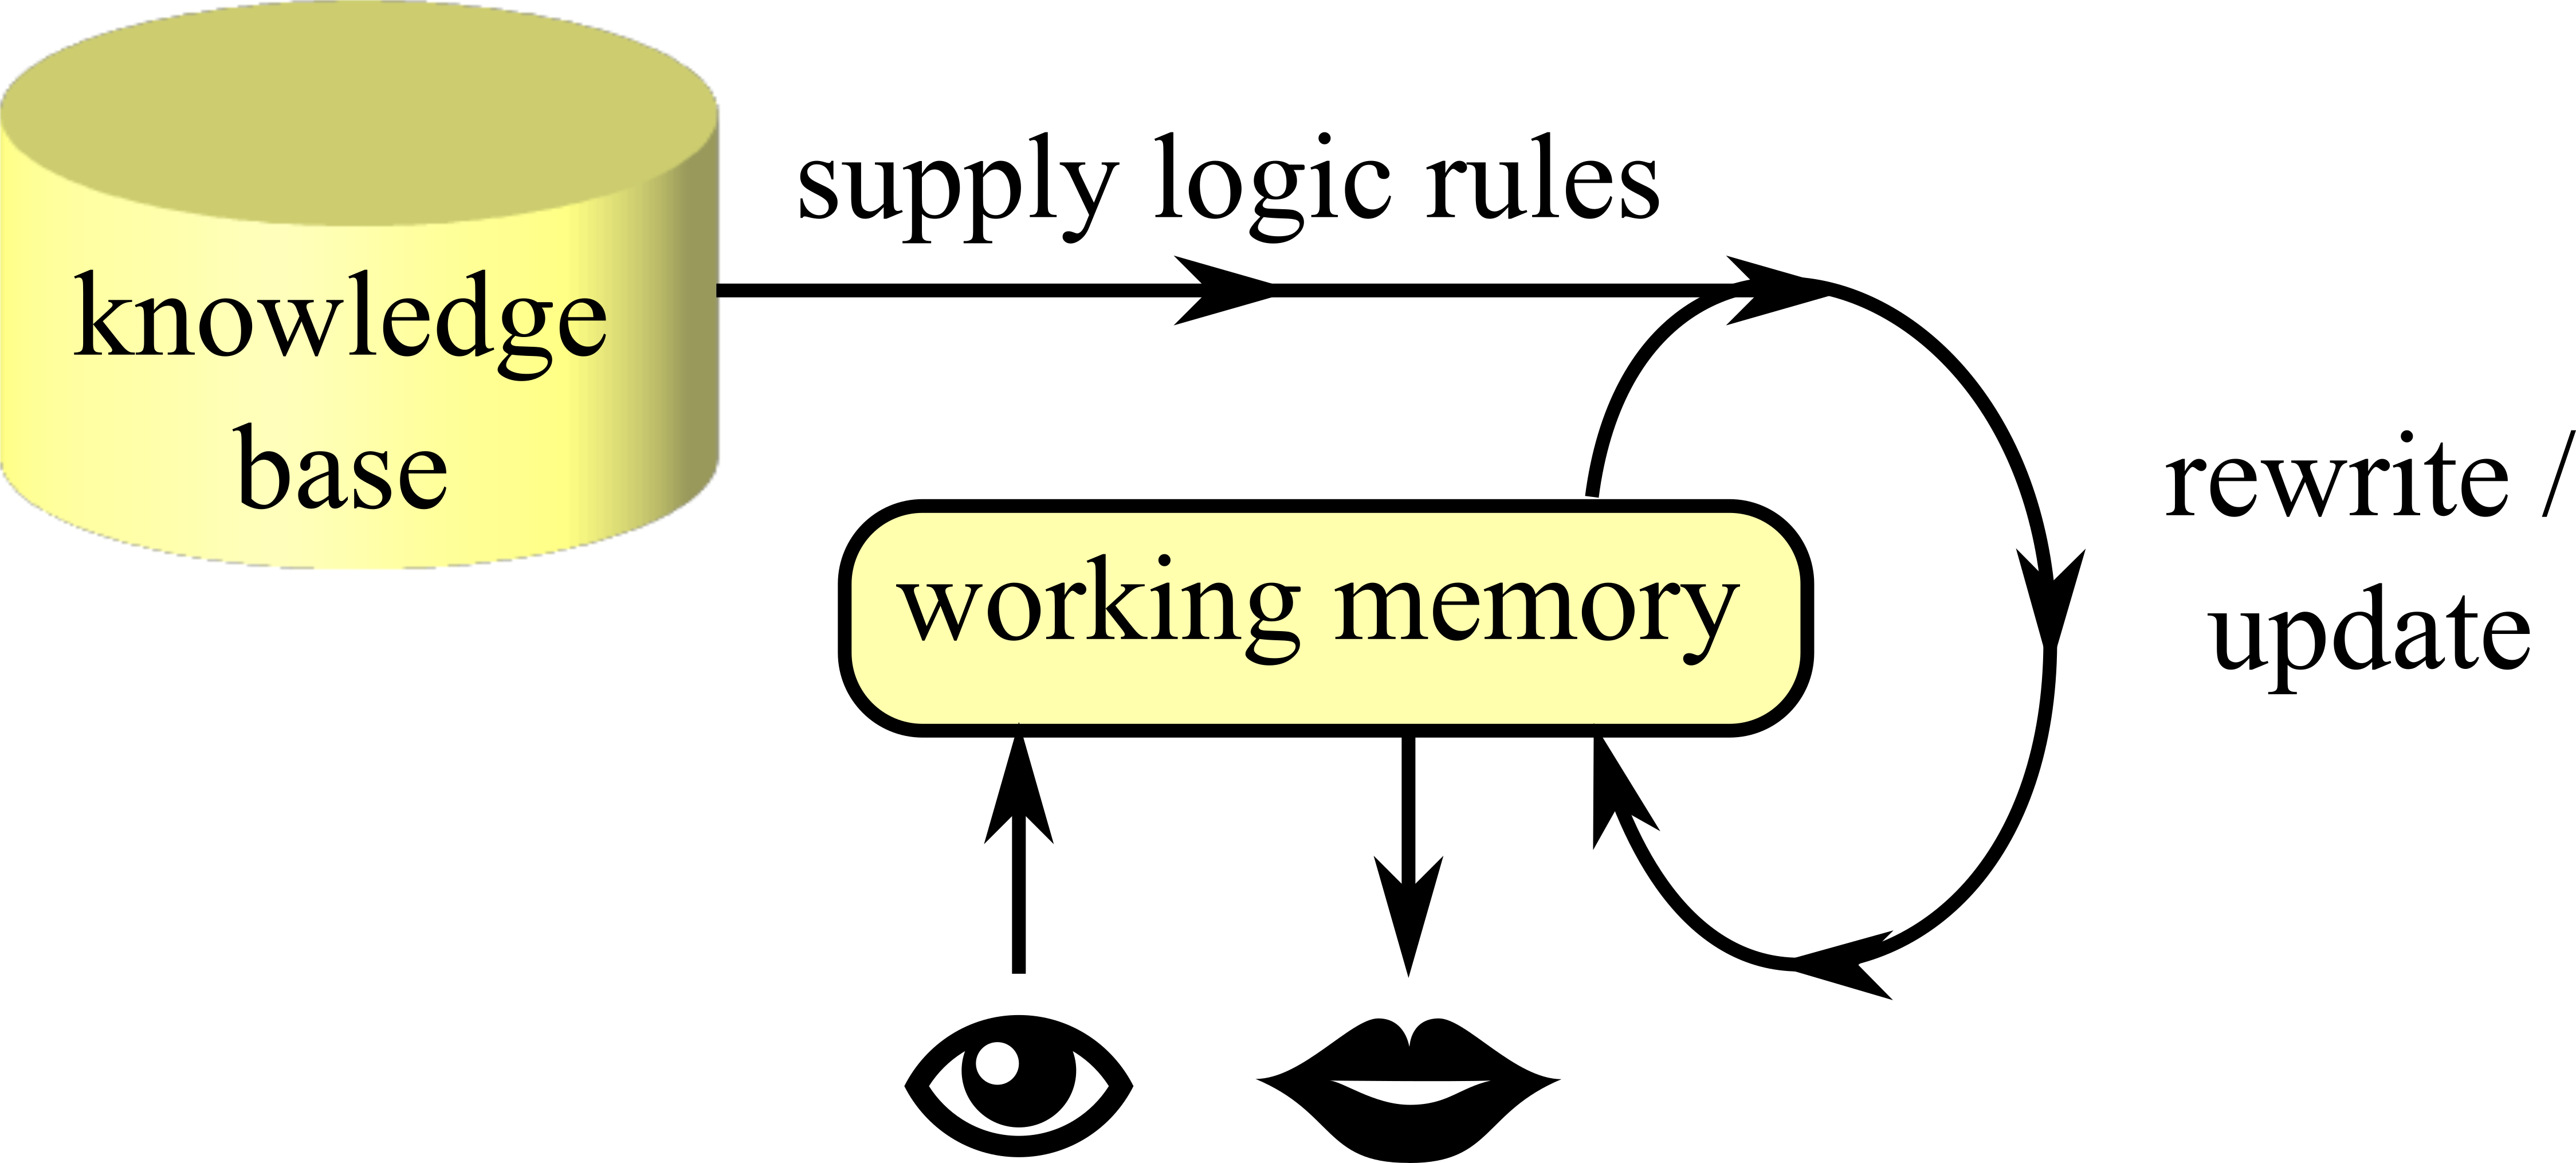
\includegraphics[scale=0.5]{LBAI-architecture.png}}}
\end{equation}
\end{frame}

\begin{frame}
\frametitle{What is a logic rule?}
\fontsize{16}{15}\selectfont
\begin{itemize}
	\item Example: loving someone and not loved back implies heartbreak:
	\begin{equation}
	\heartsuit(x,y) \wedge \neg \heartsuit(y,x) \Rightarrow \frownie{}(x)
	\end{equation}
	\item This is a rule.  Variables $x,y$ need to be {\color{red}\textbf{substituted}} with appropriate objects, \textit{eg} $\{x \setminus \mbox{John}, y \setminus \mbox{Mary} \}$
	\item Algorithm for finding substitutions is called \textbf{matching} or \textbf{unify}
\end{itemize}
\end{frame}

\begin{frame}
\frametitle{SOAR architecture}
\Wider[1em]{
\begin{itemize}
	\item is a famous \textbf{cognitive architecture}
	\item SOAR searches for logic rules that match with working memory, similar to what is depicted in (\ref{fig:LBAI-architecture})
	\item SOAR uses the \textbf{Rete} algorithm to search for applicable rules efficiently, this is an important algorithm in classical AI (\textit{rete} meaning ``web-like'' in Latin)
	% \item 鉴於中国AI的后起之秀,视野不够广阔,故补充一些基础知识
\end{itemize}
}
\end{frame}

\begin{frame}
\frametitle{My theory}
\Wider[2em]{
\begin{itemize}
	\item In my theory, the rules and their matching mechanism are \textbf{absorbed} into an NN
	\item The NN is a weapon whose strength is in approximating very complex mappings;  It is the most powerful machine-learning technology we have nowadays
	\item In my design I \textbf{relax} the structure of logic to get just the right amount of inductive bias
	\item In this design the central component is the \textbf{symmetric} NN
\end{itemize}
}
\end{frame}

\begin{frame}
\frametitle{Commutativity of logic $\wedge$}
\fontsize{16}{15}\selectfont
\Wider[1em]{
\begin{itemize}
	\item The commutativity of $\wedge$ is perhaps the most important law of logic, \textit{eg}:
	\begin{equation}
	\mbox{hungry} \wedge \mbox{penniless} \Leftrightarrow \mbox{penniless} \wedge \mbox{hungry}
	\end{equation}
	\item Could be understood as:  When deducing a conclusion from some premises, the propositions in the premise could be presented in {\color{red}\textbf{any order}}, even containing irrelevant propositions
	\item The commutative law abstracts the structure of propositions, similar to the importance of commutative groups (also called Abelian group, in memory of Abel) in abstract algebra
\end{itemize}
}
\end{frame}

\begin{frame}
\frametitle{Symmetric neural networks}
\begin{itemize}
	\item Convolutional NNs possess translational invariance
	\item Similarly, {\color{red}\textbf{symmetric}} NNs possess \textbf{permutation invariance}
	\item This can be realized via \textbf{weight-sharing}, as similar in ConvNets
	\item SymNet : logic $\approx$ ConvNet : vision
\end{itemize}
\end{frame}

\section*{Conclusion: will China build its own AGI?}

\begin{frame}
\frametitle{Will China build its own AGI?}
\fontsize{16}{15}\selectfont
\Wider[1em]{
\begin{itemize}
	\item The failure of Japan in 1980s to develop 5th-Generation computers can be a lesson
	\item As the earth has limited resources, technological progress often is the result of competition among national entities
	\item In the US there are people against China;  In China there are also people dragging our feet, supporting outsiders.  Yet I have also recieved help from American friends
	\item Therefore, I tend to be more supportive of globalized AGI projects
\end{itemize}
}
	\begin{center}
		Thanks for watching \smiley{}
	\end{center}
\end{frame}

\begin{comment}

\begin{frame}
\frametitle{References}
\footnotesize{
\begin{thebibliography}{99} % Beamer does not support BibTeX so references must be inserted manually as below
\bibitem[]{} Bart Jacobs (1999)
\newblock Categorical logic and type theory
% \newblock \emph{North Holland, Studies in logic} v141.

\bibitem[]{} Robert Goldblatt (2006)
\newblock Topoi -- the categorical analysis of logic

\end{thebibliography}
}
\end{frame}

\begin{frame}
We're looking for developers to implement a prototype.

\vspace*{1cm}
\Large{\centerline{Thank you}}

%\vspace*{1cm}
%\Large{\centerline{The End}}
\end{frame}

\end{comment}

\end{document} 